\makeatletter
\def\input@path{{../../}}
\makeatother
\documentclass[../../main.tex]{subfiles}

\graphicspath{
	{../../img/}
	{../img/}
	{img/}
}

\begin{document}
\section{Постановка задачи на условный экстремум}

В общем случае задача на условный экстремум рассматривается в 
следующем виде:

Требуется для функции $(n+m)$ переменных
\begin{equation}
\label{lec_10.num_0}
\begin{cases}
	u = f\left( x, y \right) \\
	x = \left( x_1, \ldots, x_n \right) \in D \subset \R^n \\
	y = \left( y_1, \ldots, y_m \right) \in G \subset \R^m
\end{cases}
\end{equation}
найти экстремум при наличии ограничения вида
\begin{equation}
\begin{cases} \label{lec_10.num_1}
F_k(x, y) = 0 \\
k = \overline{1, m}
\end{cases} 
\end{equation}


\begin{example}
	\;
	
	Рассмотрим Ф2П $u = x^2 + y^2$ при наличии ограничения
	$x + y = 1$, $(x, y) \in \R^2$.
	
	В данном случае, учитывая, что $y = 1 - x$, получим
	$u(x) = x^2 + (1-x)^2$. Исследуя её на локальный экстремум:
	
    \[\begin{array}{c}
	u'(x) = 2x - 2(1-x) \\
	u'(x) = 0 \implies \text{стационарная точка }x = \frac{1}{2}
	\end{array}\]
	
	$u''(\frac{1}{2}) = 4 > 0 \implies x = \frac{1}{2} = x_{min}$ функции $u(x)$.
	Тогда $y_{min} = 1 - x_{min} = \frac12$. 
	Точка 
	$M_0( \frac{1}{2}, \frac{1}{2})$~--- точка 
	условного локального минимума функции $u$, для которой 
	$u_{min} = u( \frac{1}{2}, \frac{1}{2} ) = \frac{1}{2}$. 
	
	Рассмотренный пример имеет следующую геометрическую интерпретацию:
	если $u = c \ge 0$~--- $\fix$, то получаем семейство 
	окружностей с центром в точке $(0, 0)$ и радиусом $R = \sqrt{c}$.
	Это семейство будем рассматривать в сочетании с ограничением
	$x + y = 1$, что даёт соответствующую прямую.
	Среди этих окружностей требуется выбрать ту, у которой 
	радиус либо максимален, либо минимален.
	
	В соответствующей ПДСК имеем:
	
	\begin{center}
	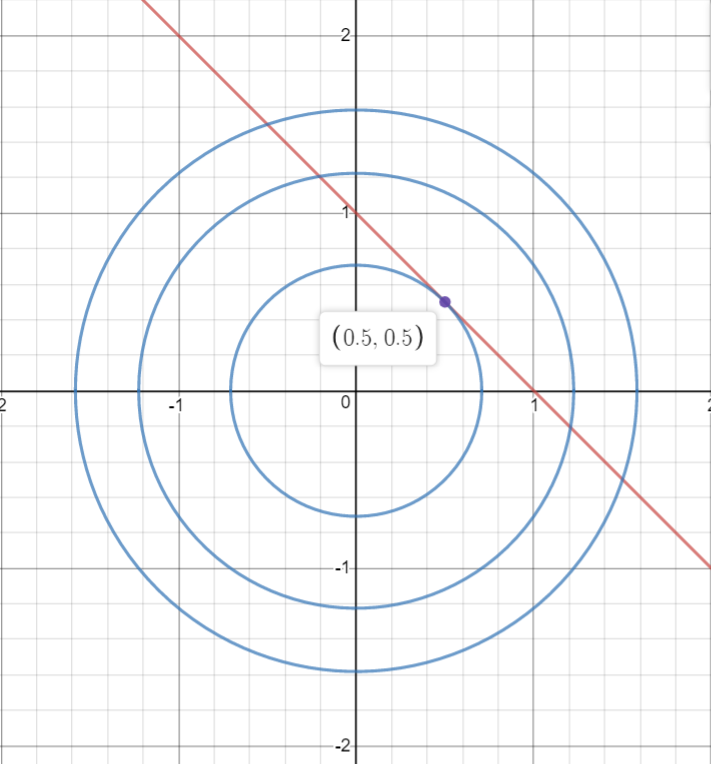
\includegraphics[width=0.6\textwidth]{family_of_circles.png}
    \end{center}
	
	Существует окружность с $R_{min} = \frac{1}{ \sqrt{2} }$, 
	которая имеет с нашей прямой одну общую точку касания: 
	$\left( \frac{1}{2}, \frac{1}{2} \right)$, т. е.
	$u_{min} = c_{min} = R^2_{min} = \frac{1}{2}$.
\end{example}

	Если обозначить $F = \left( F_1, \ldots, F_m \right) \in \R^m$, 
	то тогда \eqref{lec_10.num_1} принимает вид:
	
	\begin{equation} \label{lec_10.num_2}
		F(x, y) = \vec{0} \in \R^m.
	\end{equation}
	
	Для функции \eqref{lec_10.num_0} при ограничении \eqref{lec_10.num_2}
	точку $(x_0, y_0) \in \left( D \times G \right) 
	\subset \R^{n+m}$
	т.~е. $x_0 \in D \subset \R^n,$ $y_0 \in G \subset \R^m$ называют
	\emph{точкой условного локального экстремума} (УЛЭ) функции 
	\eqref{lec_10.num_0} при ограничении \eqref{lec_10.num_2}, если
	$\exists V( x_0, y_0 ) \subset D \times G $ такая, что 
	$\forall ( x, y) \in V( x_0, y_0) \implies $
	
	\begin{itemize}
		\item[a)] 
		$F(x_0, y_0) = 0$
		\item[б)]
		$\left[ \begin{gathered}
		f(x,y) \ge f(x_0, y_0)\text{~--- локальный минимум} \\
		f(x, y) \le f(x_0, y_0)\text{~--- локальный максимум} 
		\end{gathered} \right.$
	\end{itemize}
		
Предположим, что используемые функции $F_k(x,y),\ k = \overline{1, m}$ 
непрерывно дифференцируемы по своим переменным. В этом случае для 
матрицы Якоби имеем:

\begin{equation} \label{lec_10.num_3}
	\rank \left.\begin{bmatrix}
	\pderiv{F_1}{x_1} & \ldots & \pderiv{F_1}{x_n} & 
	\pderiv{F_1}{y_1} & \ldots & \pderiv{F_1}{y_m} \\
	\pderiv{F_2}{x_1} & \ldots & \pderiv{F_2}{x_n} &
	\pderiv{F_2}{y_1} & \ldots & \pderiv{F_2}{y_m} \\
	\vdots & \ddots & \vdots & \vdots & \ddots & \vdots \\
	\pderiv{F_m}{x_1} & \ldots & \pderiv{F_m}{x_n} &
	\pderiv{F_m}{y_1} & \ldots & \pderiv{F_m}{y_m}
	\end{bmatrix}
	\right|_{(x_0, y_0)} = m
\end{equation} 		
		
Тогда без ограничения общности можно считать, что минор
$r$-го порядка, расположенный в последних столбцах, ненулевой, т.е

\begin{equation} \label{lec_10.num_4}
	I_0 = \det \begin{bmatrix}
	\pderiv{F_1}{y_1} & \ldots & \pderiv{F_1}{y_m} \\
	\vdots & \ddots & \vdots \\
	\pderiv{F_m}{y_1} & \ldots & \pderiv{F_m}{y_m}
	\end{bmatrix} \ne 0.
\end{equation}

По теореме об однозначной разрешимости СФУ получаем, что 
соотношение \eqref{lec_10.num_2} разрешимо относительно $y = \left( 
y_1, \ldots, y_m \right)$ в соответствующей $\widetilde{V} (x_0, y_0)$.
При этом получаемые решения $y_k = y_k \left( x_1, \ldots, x_n 
\right),\ k = \overline{1, m}$ будут удовлетворять начальному условию
$y(x_0) = \left( y_1(x_0), \ldots, y_m(x_0) \right) = y_0$.

В связи с этим для полученного решения $y = \varphi(x) = \left( 
y_1(x), \ldots, y_m(x) \right)$ после подстановки в \eqref{lec_10.num_0} 
приходим к $u(x) = f( x, \varphi(x) ), x \in \widetilde{V}(x_0)$, 
исследования которой на обычный локальный экстремум будут 
соответствовать исследованию \eqref{lec_10.num_0} 
при ограничениях \eqref{lec_10.num_2} на условный локальный экстремум.
Т.е задача на условный локальный экстремум сводится, при возможности, 
к задаче на безусловный 
локальный экстремум, что было сделано в предыдущем примере.

\section{Метод дифференциалов исследования на условный локальный экстремум}

Предполагая непрерывную дифференцируемость функций связи \eqref{lec_10.num_2} 
в $V(x_0, y_0)$ и считая выполенным \eqref{lec_10.num_4}, как и выше,
получаем однозначную разрешимость \eqref{lec_10.num_2}, т.е
\[\exists\:y = \varphi(x) \implies F( x, \varphi(x)) \equiv 0,\ 
y_0 = \varphi(x_0).\]

После подстановки для
\begin{equation} \label{lec_10.num_5}
	u = f( x, \varphi(x) )
\end{equation}
в силу необходимого условия обыкновенного локального экстремума 
рассматриваемой точки $(x_0, y_0)$ имеем:
\[ du(x_0, y_0) = 0. \]
Отсюда, в силу инвариантности формы первого дифференциала для 
$\Phi(x) = f( x, \varphi(x) )$:

\begin{equation} \label{lec_10.num_6}
	d\Phi(x_0) = \sum_{k = 1}^{n} \pderiv{ f(x_0, y_0) }{x_k} 
	dx_k + \sum_{j = 1}^{m} \pderiv{ f(x_0, y_0) }{y_j} dy_j = 0.
\end{equation}

Рассматривая \eqref{lec_10.num_6} как линейную систему относительно неизвестных
$d\varphi_1, \ldots, d\varphi_m$ и учитывая, что якобиан 
этой системы не равен $0$,
мы можем однозначно выразить линейным образом $d\varphi_1, \dots, d\varphi_m$
через независимые дифференциалы $dx_1, \ldots, dx_n$.

В результате получаем, что в рассматриваемой точке $(x_0, y_0)$,
являющейся стационарной для $u = u\left( x, \varphi(x) \right)$:
\[ du(x_0, y_0) = 0, \]
что после подстановки зависимых $d\varphi_j$ через независимые 
$dx_1, \ldots, dx_n$, приводит к виду:

\begin{equation} \label{lec_10.num_7}
	\sum_{k = 1}^{n} A_k dx_k = 0,\ A_k = A_k(x_0, y_0) \in \R.
\end{equation}
Из \eqref{lec_10.num_7} в силу независимости используемых дифференциалов 
$\implies \forall A_k = 0,\ k = \overline{1, n}$

Присоединяя уравнение связи точки $(x_0, y_0)$, получаем 
соответствующую систему для стационарной точки локального 
условного экстремума вида:
\[ \begin{cases}
	F_j(x_0, y_0) = 0, \; j = \overline{1, m} \\
	A_k(x_0, y_0) = 0, \; k = \overline{1, n}
\end{cases} \]
Здесь система из $(n+m)$ уравнений относительно $(n+m)$ неизвестных.

На практике основная трудность~--- решение этой системы.
Решив её, полученную стационарную точку $(x_0, y_0)$ исследуют
на обыкновенный локальный экстремум обычным образом.

\begin{example}
	\;
	
	Рассмотрим функцию 
	\[ \begin{cases}
	u = x - 2y + 2z \\
	F = x^2 + y^2 + z^2 -1 = 0
	\end{cases} \]
	
	Имеем:
	\[\begin{array}{l}
	du = dx - 2dy + 2dz \\
	dF = 2xdx + 2ydy + 2zdz = 0
	\end{array}\]
	
	Считая, что $z \ne 0$:
	\[dz = -\dfrac{x}{2}dx - \dfrac{y}{2}dy\]
	
	Отсюда
	\[du = dx - 2dy + 2\left( -\dfrac{x}{2}dx - 
	\dfrac{y}{2} dy \right) = 
	\left( 1 - \dfrac{2x}{z} \right)dx - 
	2\left( 1 + \dfrac{y}{z} \right)dy.\]
	
	Решая уравнение $du = 0$ и учитывая независимость $dx$ и $dy$,
	получаем систему
	
	\[
	\begin{cases}
	A_1 = 1 - \dfrac{2}{z} = 0 \\
    \\
	A_2 = 1 + \dfrac{y}{z} = 0 \\
	x^2 + y^2 + z^2 - 1 = 0
	\end{cases} 
	\]
	
	Отсюда
	\[ \begin{cases}
	z = 2x \\
	y = -z = -2x \\
	x^2 + 4x^2 + 4x^2 = 1
	\end{cases} \]
	
	\[x^2 = \dfrac{1}{9} \implies
	 \begin{cases}
        x = \pm \dfrac{1}{3} \implies \\
        y = -2x = \mp \dfrac{2}{3} \\
        z = 2x = \pm \dfrac{2}{3}
	 \end{cases}
	\]
 
	Мы нашли две точки локального экстремума: $M_{1,2} 
	\left( \pm \dfrac{1}{3}, \mp \dfrac{2}{3}, 
	\pm \dfrac{2}{3} \right)$ Для исследования их на экстремальность, выразим $d^2 u$ через
	независимые $dx$ и $dy$:
\end{example}

\end{document}
